\chapter{Evaluácia výsledkov}

\paragraph{}
V predošlej kapitole sme bližšie popísali implementáciu našich algoritmov. Táto kapitola sa zameriava na evaluáciu výsledkov z týchto algoritmov. Keďže celá táto práca sa zaoberá implementáciou algoritmov na generovanie hesiel pomocou vstupného slovníka, bolo potrebné si nájsť vhodný vstupný slovník. Podarilo sa nám nájsť online zdroj slovníkov \cite{dictionaries}, ktorý obsahuje slovníky s usporiadanými heslami podľa pravdepodobnosti výskytu. Slovník je formátovaný v dvoch stĺpcoch, kde prvý obsahuje informáciu o počte výskytov daného heslá a druhý je samotné heslo.

\section{Časová náročnosť}
\label{sec:time}
V tomto základnom teste sme spustili naše algoritmy a merali čas behu algoritmov pre jednotlivé parametre spustenia. Pre všetky testy používame slovník \emph{phpbb} stiahnutý z \cite{dictionaries}. Slovník sme upravovali aby obsahoval len heslá zodpovedajúce maximálnej dĺžke hesiel, ktoré generuje bezkontextová gramatika. Týmto sme znížili pravdepodobnosť Markovovského zdroja generovať heslá dlhšie ako stanovené maximum pre gramatiku. Stĺpec \emph{d} označuje maximálnu dĺžku generovaných hesiel zatiaľ čo stĺpec \emph{p} vyjadruje maximálnu veľkosť jednoduchého neterminálu v prípade bezkontextovej gramatiky zatiaľ čo pri Markovovskom zdroji vyjadruje dĺžku prefixu podľa ktorého sa rozhoduje. Tieto časové testy boli spúšťané na procesore Intel® Core™ i5-4690K s rýchlosťou 3.50GHz na operačnom systéme Windows 10. Namerané hodnoty zobrazené v tabuľke sú uvedené v sekundách.

\begin{table}[]
\centering
\caption{Časy pre slovník phpbb}
\label{tphpbb}
\begin{tabular}{lll|lllllll}
       & d & p & GEN     & 10000  & 50000  & 100000 & 500000 & 1000000 & 5000000 \\ \hline
CFG    & 6 & 2 & 0.103   & 0.754  & 3.504  & 7.097  & 35.109 & 71.129  & 369.057 \\
CFG    & 6 & 3 & 0.32    & 2.696  & 5.441  & 9.028  & 37.121 & 72.181  & 354.763 \\
CFG    & 6 & 4 & 6.053   & 2.621  & 5.53   & 8.96   & 37.515 & 73.744  & 367.655 \\
CFG    & 6 & 5 & 156.141 & 47.595 & 50.767 & 54.054 & 81.957 & 116.699 & 397.522 \\
Markov & 6 & 2 & ---     & 1.284  & 3.936  & 7.469  & 34.533 & 68.029  & 337.949 \\
Markov & 6 & 3 & ---     & 2.218  & 4.839  & 8.28   & 35.406 & 69.88   & 347.756 \\
Markov & 6 & 4 & ---     & 4.833  & 7.926  & 10.874 & 38.463 & 81.074  & 373.771 \\ \hline
       & d & p & GEN     & 10000  & 50000  & 100000 & 500000 & 1000000 & 5000000 \\ \hline
CFG    & 7 & 2 & 0.21    & 0.808  & 3.646  & 7.011  & 35.11  & 70.911  & 361.186 \\
CFG    & 7 & 3 & 0.419   & 0.84   & 3.607  & 7.156  & 36.138 & 71.242  & 361.462 \\
CFG    & 7 & 4 & 6.182   & 3.022  & 5.459  & 9.041  & 37.589 & 73.397  & 364.075 \\
CFG    & 7 & 5 & 158.024 & 53.649 & 52.981 & 56.456 & 84.178 & 119.034 & 402.945 \\
Markov & 7 & 2 & ---     & 1.648  & 4.361  & 7.753  & 34.48  & 68.228  & 349.683 \\
Markov & 7 & 3 & ---     & 2.864  & 5.575  & 9.602  & 37.016 & 71.108  & 346.98  \\
Markov & 7 & 4 & ---     & 8.19   & 10.772 & 13.921 & 43.673 & 79.005  & 379.443 \\ \hline
       & d & p & GEN     & 10000  & 50000  & 100000 & 500000 & 1000000 & 5000000 \\ \hline
CFG    & 8 & 2 & 0.588   & 0.905  & 3.662  & 7.094  & 36.179 & 71.394  & 369.456 \\
CFG    & 8 & 3 & 0.818   & 0.939  & 3.71   & 7.338  & 36.871 & 74.814  & 362.259 \\
CFG    & 8 & 4 & 6.758   & 3.015  & 5.182  & 8.512  & 34.945 & 68.242  & 335.426 \\
CFG    & 8 & 5 & 159.983 & 51.749 & 49.595 & 53.055 & 78.314 & 110.507 & 374.249 \\
Markov & 8 & 2 & ---     & 2.462  & 5.029  & 8.441  & 34.9   & 68.778  & 337.725 \\
Markov & 8 & 3 & ---     & 4.679  & 7.333  & 10.563 & 38.329 & 71.626  & 345.412 \\
Markov & 8 & 4 & ---     & 12.857 & 16.485 & 24.572 & 54.914 & 87.455  & 428.908
\end{tabular}
\end{table}

\begin{figure}[ht]
    \centering
    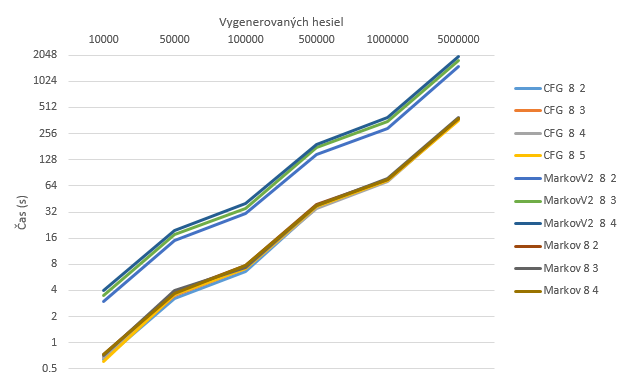
\includegraphics[width=1\textwidth]{generateTime}
    \caption{Čas generovania hesiel}
    \label{fig:generateTime}
\end{figure}

\paragraph{}
\section{Výstupné heslá}
\label{sec:pass}
Po overení časovej zložitosti generovania hesiel pomocou jednotlivých algoritmov sme na výsledné heslá aplikovali viaceré metriky. Cieľom týchto testov bolo ukázať výhody a slabiny jednotlivých algoritmov a spraviť ich vzájomne porovnanie v zmysle šancí na nájdenie hľadaného heslá. Vzhľadom na to, že v praxi sa trendy medzi používanými heslami môžu meniť a časom by mohla drvivá väčšina ľudí používať bezpečné heslá, tieto metriky nie sú záväzne a nevypovedajú o tom ako sa budú jednotlivé algoritmy správať ak by boli použité v praxi.

\subsection{Heslá zo vstupného slovníka}
Ako prvú metriku sme skúmali koľko hesiel zo slovníka gramatika vygenerovala po vygenerovaní určitého počtu hesiel. Na grafoch, ktoré boli výstupom tohto testu sme na vodorovnej osi znázornili počet hesiel vygenerovaných gramatikou v tisícoch zatiaľ čo na vertikálnej osi je percento hesiel slovníka, ktoré sa medzi nimi nachádzajú. Pri tomto teste sme nechali oba algoritmy generovať 100 miliónov hesiel k čomu bol použitý slovník obsahujúci 13 331 008 rôznych hesiel dĺžky 12 a menej znakov.

\paragraph{}
Nižšie vidíme grafy znázorňujúce vývoj počtu vygenerovaných hesiel, ktoré sa nachádzajú v slovníku. Zatiaľ čo prvý zobrazuje koľko unikátnych hesiel bolo vygenerovaných pomocou algoritmu využívajúceho Markovovské zdroje, tie následovne ukazujú vyššie popísanú metriku ohľadom počtu vygenerovaných hesiel patriacich do vstupného slovníka.

\begin{figure}[ht]
    \centering
    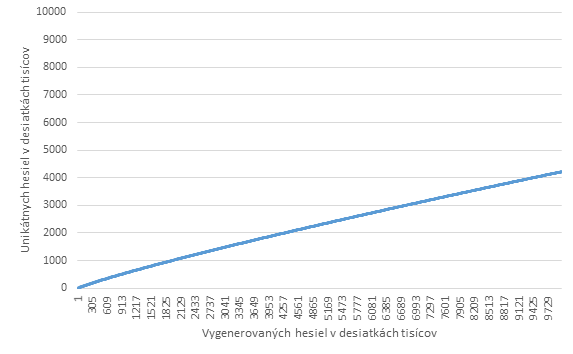
\includegraphics[width=1\textwidth]{uniqMarkov}
    \caption{Počet unikátnych hesiel}
    \label{fig:uniqMarkov}
\end{figure}
\paragraph{Heslá zo vstupného slovníka}
Na \ref{fig:sameDictAcc} vidíme priebeh hodnôt, kde heslá boli porovnávané so vstupným slonvíkom. Vidíme, že nami definované a implementované riešenie pomocou bezkontextových gramatík má na rozdiel od Markovovského zdroja omnoho pomalší rast počtu hesiel patriacich do slovníka. Pri 100 miliónoch generovaných hesiel to je niečo málo pod 700 tisíc. Dôvod pre takéto relatívne malé percento vygenerovaných hesiel zo slovníka môže byť práve vlastnosť gramatiky učiť sa vzory hesiel. Keďže vo vstupnom slovníku existovalo málo hesiel, ktoré mali obrovský počet výskytov, gramatika sa zamerala na generovanie hesiel s veľmi podobným vzorom.

\begin{figure}[ht]
    \centering
    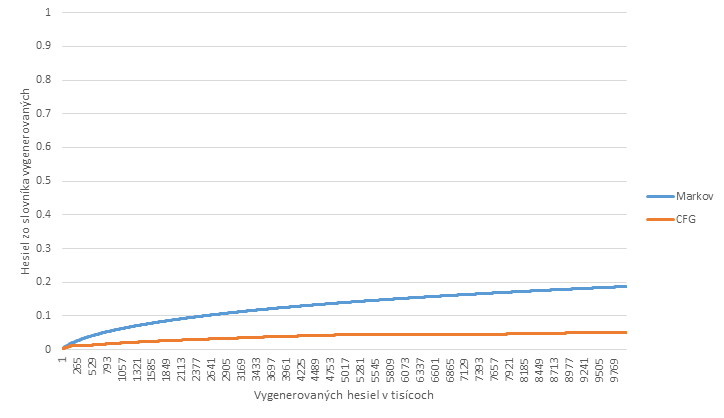
\includegraphics[width=1\textwidth]{sameDictAcc}
    \caption{Pomer vygenerovaných hesiel zo vstupného slovníka}
    \label{fig:sameDictAcc}
\end{figure}

\paragraph{Heslá z nezávislého slovníka}
Graf \ref{fig:otherDictAcc} znázorňuje hodnoty po porovnaní vygenerovaných hesiel s iným nezávislým slovníkom. Pri tomto teste sme zobrali heslá vygenerované našimi algoritmami, ktoré na vstupe dostali slovník \emph{rockyou}. Následne sme spravili testy počtu vygenerovaných hesiel, tentokrát avšak z iného ako vstupného slovníka. V tomto prípade sme použili slovník \emph{phpbb}. Týmto by sme chceli ukázať schopnosť nášho algoritmu vygenerovať slovník veľmi podobný tým používaným v praxi.

\begin{figure}[ht]
    \centering
    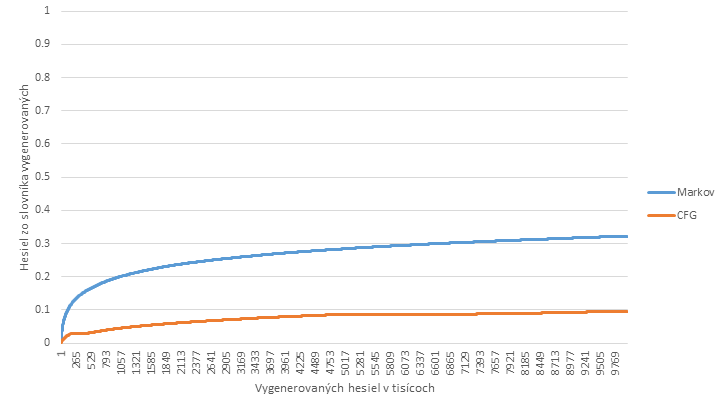
\includegraphics[width=1\textwidth]{otherDictAcc}
    \caption{Pomer vygenerovaných hesiel z nezávislého slovníka}
    \label{fig:otherDictAcc}
\end{figure}

Ďalej sme taktiež skúmali ako sa správajú nami implementované algoritmy ma menších dátach. Na obrázku \ref{fig:Acc6} je znázornený graf priebehu generovania hesiel, ktoré sa nachádzajú vo vstupnom slovníku. Na vodorovnej osi je ukázaný počet vygenerovaných hesiel, v tomto prípade to bolo 5 miliónov hesiel. Výška čiar určuje množstvo hesiel, ktoré boli nájdene vo vstupnom slovníku. Pre Markovovské zdroje sa toto číslo počíta z počtu unikátnych hesiel, ktoré boli vygenerované. Všimli sme si, že priebehy jednotlivých algoritmov sa náramne podobajú logaritmickej krivke. Taktiež si môžme všimnúť, že algoritmus používajúci Markovovské zdroje je v tejto metriky opäť lepší ako algoritmus používajúci pravdepodobnostné bezkontextové gramatiky. Použili sme slovník \emph{phpbb} stiahnutý z \cite{dictionaries}, ktorý sme upravili aby všetky heslá mali dĺžku najviac 6 znakov. Takto upravený slovník mal nakoniec 55 744 rôznych hesiel.

\begin{figure}[ht]
    \centering
    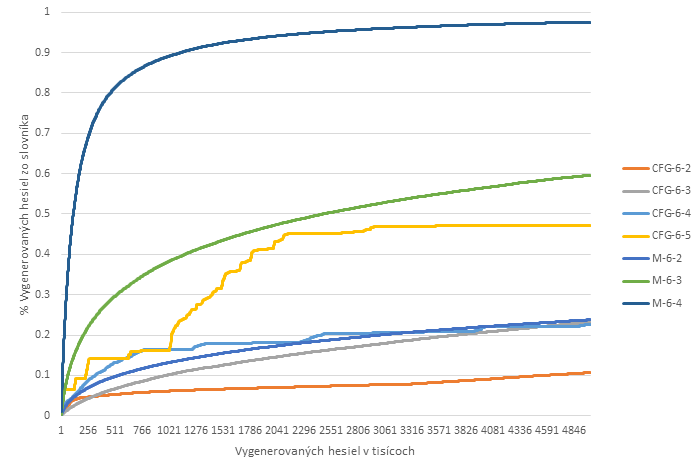
\includegraphics[width=1\textwidth]{sameDictAcc6}
    \caption{Počet vygenerovaných hesiel zo slovníka - dĺžka 6}
    \label{fig:Acc6}
\end{figure}

Po zhliadnutí rovnakého grafu pre algoritmy pustené pre generovanie hesiel dĺžky 7 a s upraveným slovníkom phpbb obsahujúcim heslá najviac dĺžky 7 sme si všimli, že množstvo hesiel zo vstupného slovníka generovaných našimi algoritmami sa nezmenilo až na Markovovské zdroje s prefixom 4. V tomto teste bola veľkosť vstupného slovníka 88 416 hesiel.

\begin{figure}[ht]
    \centering
    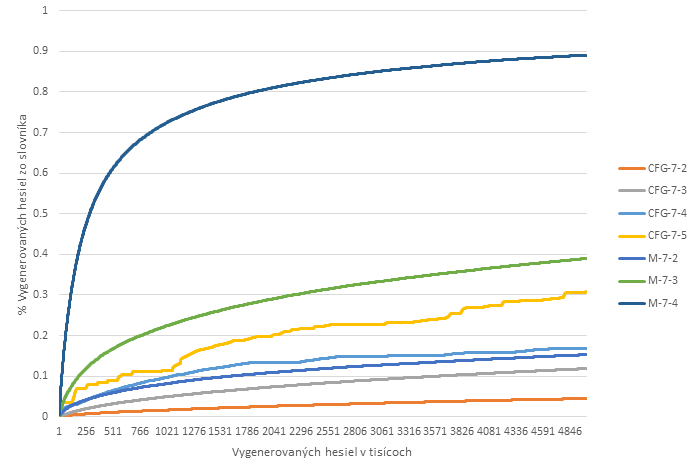
\includegraphics[width=1\textwidth]{sameDictAcc7}
    \caption{Počet vygenerovaných hesiel zo slovníka - dĺžka 7}
    \label{fig:Acc7}
\end{figure}

Nakoniec sme tento istý test opäť spustili na všetkých algoritmoch. Tentokrát vstupné parametre a slovník boli nastavené na generovanie hesiel maximálnej dĺžky 8. Takto upravený slonvík phpbb obsahoval 143 675 hesiel z ktorých až 100 tisíc bolo vygenerovaných algoritmom používajúcim Markovovské zdroje s prefixom nastaveným na dĺžku 4. V grafe zobrazujúci tieto dáta sme zobrazili výsledky tohto testu aj pre nami upravenú verziu Markovovských zdrojov, ktorá by mala byt schopná v konečnom čase vygenerovať heslá z celého priestoru možností. Označili sme ju ako \emph{M2-8-4} keďže sa jedná o druhú verziu Markovovských zdrojov použitých v tejto práci.

\begin{figure}[ht]
    \centering
    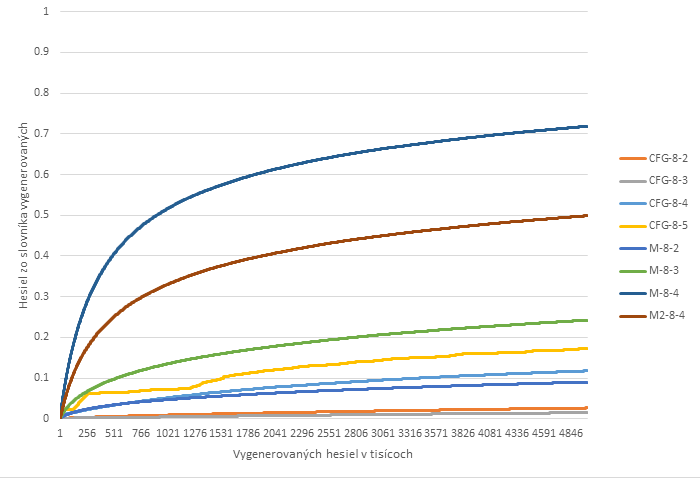
\includegraphics[width=1\textwidth]{sameDictAcc8}
    \caption{Počet vygenerovaných hesiel zo slovníka - dĺžka 8}
    \label{fig:Acc8}
\end{figure}

\paragraph{}
V prípade nami upraveného Markovovského zdroja a algoritmu, ktorý ho používa pri generovaní hesiel sme taktiež testovali vplyv nastavenie konštánt \(\delta\) a \(\varepsilon\). V následujúcom grafe \ref{fig:MarkovV2} zobrazujeme rozdiel v počte vygenerovaných hesiel zo vstupného slovníka pre jednotlivé parametre označené v legende grafu ako \(\delta-\varepsilon\). Vidíme, že tieto parametre nemajú žiaden vplyv na prvých 5 miliónov hesiel vygenerovaných týmto algoritmom.

\begin{figure}[ht]
    \centering
    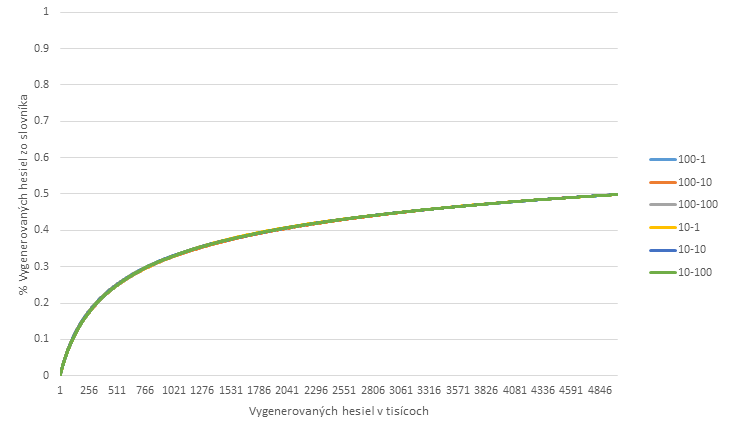
\includegraphics[width=1\textwidth]{sameDictAccMarkv2}
    \caption{Počet vygenerovaných hesiel zo slovníka - dĺžka 8}
    \label{fig:MarkovV2}
\end{figure}

\paragraph{}
Na základe \ref{fig:sameDictAcc} a \ref{fig:otherDictAcc} vidíme, že nami navrhnutá metóda pomocou bezkontextových gramatík síce negeneruje veľa hesiel zo vstupného slovníka počas prvých miliónov vygenerovaných hesiel. Tento problém by sa dal vyriešiť, tým že by sme vždy ako prvé na výstup poslali všetky heslá zo slovníka, keďže ten býva zanedbateľne malý oproti veľkosti priestoru hesiel, ktorý musíme prehľadať aby sme definitívne našli hľadané heslo.

\subsection{Miery presnosti}
Pod týmto pojmom rozumieme metriky popisujúce nielen kvantitu nami generovaných hesiel patriacich do slovníka, ale snažia sa bližšie vyhodnotiť ako rýchlo sa gramatika dostane k heslám, ktoré boli podľa vstupného slovníka označené za najpravdepodobnejšieho.

\paragraph{}
Stĺpce tabuľky \ref{mieryPresnosti} vyjadrujú hodnoty jednotlivých metrík pre daný algoritmus.
\begin{itemize}
	\item \emph{PPS} - Priemerná Pozícia v Slovníku - Vyjadruje priemernú pozíciu vo vstupnom slovníku hesiel, ktoré boli vygenerované algoritmom na výstupe
	\item \emph{PPS \%} - Priemerná Pozícia v Slovníku - Vyjadruje percentuálnu pozíciu vrámci slovníku hesiel, ktoré boli vygenerované algoritmom na výstupe
	\item \emph{RPSV} - Rozdiel Pozície v Slovníku a na Výstupe - Rozdiel v pozícií na vstupe a na výstupe algoritmu prenásobený percentuálnym počtom výskytov vo vstupnom slovníku
    \item \emph{OPSV} - Odchýlka Pozície v Slovníku a na Výstupe - Absolútna hodnota rozdielu v pozícií na vstupe a na výstupe algoritmu prenásobená percentuálnym počtom výskytov vo vstupnom slovníku
\end{itemize}

\[ \frac{\displaystyle\sum_{i=1}^{k}((indG_i - indS_x) * \frac{v_{ind_x}}{\sum_{j=1}^{n}v_j})}{k} \]

Vzorec vyjadrujúci mieru RPSV, kde \emph{n} vyjadruje počet hesiel vo vstupnom slovníku a \emph{k} je počet výskytov hesiel zo vstupného slovníka medzi generovanými. Hodnota \emph{\(indG_i\)} určuje poradie i-tého heslá nachádzajúceho sa vo vstupnom aj výstupnom slovníku vrámci generovaného slovníka. Hodnota \emph{\(indS_i\)} vyjadruje tú istú hodnotu pre vstupný slovník. Hodnoty \emph{\(v_i\)} sú počty výskytov hesiel zadefinované vo vstupnom slovníku.

\paragraph{}
Vzorec pre mieru OPSV je takmer identický s vyššie uvedeným vzorcom, jediný rozdiel je v absolútnej hodnote rozdiel medzi pozíciami na vstupe a výstupe.

\[ \frac{\displaystyle\sum_{i=1}^{k}(|indG_i - indS_x| * \frac{v_{ind_x}}{\sum_{j=1}^{n}v_j})}{k} \]

\paragraph{}
Priemerná pozícia v slovníku ukazuje ako pravdepodobné heslá v priemernom prípade generuje náš algoritmus. Keďže toto číslo sa často krát zdá veľké, prikladáme k nemu v druhom stĺpci jeho percentuálnu hodnotu. Hodnoty d a p vyjadrujú maximálnu dĺžku hesiel v slovníku a dĺžku použitých prefixov v Markovovskom zdroji. Pre hodnoty 6,7,8 parametru \emph{d} sme použili slovník \emph{phppbb} upravený na heslá relevantnej dĺžky. Pre hodnoty \emph{d} rovné 12 sme použili omnoho robustnejší slovník \emph{rockyou}, skladajúci sa z takmer 14 miliónov unikátnych hesiel.

\begin{table}[]
\centering
\caption{Miery presnosti}
\label{mieryPresnosti}
\begin{tabular}{lll|llll}
       & d  & p & PPS & PPS \% & RPSV  & OPSV\\ \hline
CFG    & 6  & 2 & 31328    & 56.1       & 36.567 & 36.671    \\
CFG    & 6  & 3 & 26358    & 47.2       & 37.749 & 37.762    \\
CFG    & 6  & 4 & 31033    & 55.6       & 19.673 & 19.725    \\
CFG    & 6  & 5 & 28554    & 51.2       & 21.397 & 21.484    \\
CFG    & 7  & 2 & 47454    & 53.6       & 26.489 & 26.531    \\
CFG    & 7  & 3 & 40343    & 45.6       & 25.831 & 25.848    \\
CFG    & 7  & 4 & 46739    & 52.8       & 16.648 & 16.700    \\
CFG    & 7  & 5 & 46718    & 52.8       & 21.715 & 21.804    \\
CFG    & 8  & 2 & 88521    & 61.6       & 16.139 & 16.199    \\
CFG    & 8  & 3 & 61113    & 42.5       & 22.384 & 22.436    \\
CFG    & 8  & 4 & 70500    & 49.0       & 15.028 & 15.071    \\
CFG    & 8  & 5 & 75570    & 52.5       & 14.749 & 14.865    \\
Markov & 6  & 2 & 25219    & 45.2       & 28.307 & 28.332    \\
Markov & 6  & 3 & 25959    & 46.5       & 14.815 & 14.840    \\
Markov & 6  & 4 & 27705    & 49.7       & 3.649 & 3.706    \\
Markov & 7  & 2 & 39090    & 44.2       & 21.289 & 21.323    \\
Markov & 7  & 3 & 40283    & 45.5       & 13.321 & 13.353    \\
Markov & 7  & 4 & 43232    & 48.8       & 4.700 & 4.757    \\
Markov & 8  & 2 & 61688    & 42.9       & 15.745 & 15.792    \\
Markov & 8  & 3 & 66401    & 46.2       & 9.701 & 9.748    \\
Markov & 8  & 4 & 68291    & 47.5       & 4.596 & 4.658    \\ \hline \hline
CFG    & 12 & 4 & 3781788    & 28.3       & 5.879 & 5.925    \\
Markov & 12 & 4 & 4609712    & 34.5       & 2.191 & 2.224   
\end{tabular}
\end{table}

\paragraph{}
Z tabuľky \ref{mieryPresnosti} môžme vidieť že obom našim algoritmom prospieva navýšenie vstupnej informácie o heslách. Toto je vidieť na jak na percentuálnych hodnotách priemernej pozície v slovníku tak aj na rozdieloch pozícií medzi vstupným a vygenerovaným slovníkom. Hodnota rozdielov pozícií má vyjadrovať presnosť generovania hesiel v správnom poradí kedy algoritmus je odmenený znížením skóre ak sa mu podarí vygenerovať niektoré heslo skôr ako sa nachádza vo vstupnom slovníku. Posledná miera \emph{odchýlka pozície v slovníku} má vyjadrovať absolútny rozdiel pozícií oproti vstupnému slovníku bez ohľadu na to, či heslo bolo vygenerované skôr ako vo vstupnom slovníku. Malý rozdiel týchto hodnôt naznačuje, že väčšina hesiel, ktoré boli generované našimi algoritmami bola vygenerovaná neskôr ako bol jej výskyt vo vstupnom slovníku.